

\section{Introduction}
The range of bacterial growth rates can be enormous. In natural environments,
some microbial organisms might double only once per year, whereas in comfortable
laboratory conditions growth can be rapid with several divisions per hour. This
remarkable diversity illustrates the intimate relationship between environmental
conditions and the rates at which cells convert nutrients into new cellular
material. This relationship between the environment and cellular growth rate has
remained a major topic of inquiry in bacterial physiology for over a century
\citep{jun2018}. In 1958, Schaecter, Mall\o e, and Kjeldgaard reported the
discovery of a logarithmic relationship between the total cellular protein
content and the cellular growth rate, revealing a fundamental relationship
between the environment and the composition of the intracellular milieu
\citep{schaechter1958}.

Over the past decade, a remarkable body of work has reexamined this relationship
with single-cell and single-protein resolution using modern methods of video
microscopy \citep{si2017,harris2018} and through advances in mass spectrometry and
sequencing technologies \citep{schmidt2016,li2014}. This has permitted
quantitative insight into how bacteria like \textit{E. coli} allocate their
cellular resources under nutrient-limitation, and following genomic and
pharmacological perturbations \citep{scott2010,hui2015,basan2015}.
This body of experimental data places us in the auspicious position to
explore how the abundance of essential protein complexes are related to the
growth rate of the population and interrogate what biological processes may set
the speed limit of bacterial growth.

In this work, we seek to leverage a collection of proteomic data sets of
\textit{Escherichia coli} across 31 growth conditions \citep{valgepea2013,li2014,
peebo2015,hui2015,schmidt2016} to quantitatively explore what biological
processes may set the speed limit of bacterial growth. Broadly speaking, we
entertain several classes of hypotheses as are illustrated in \FIG{categories}.
First, we consider potential limits on the transport of nutrients into the cell.
We address this hypothesis by performing an order-of-magnitude estimate for how
many carbon atoms needed to facilitate this requirement given a 6000 second
division time.  As a second hypothesis, we consider the possibility that there
exists a fundamental limit on how quickly the cell can generate ATP. We approach
this hypothesis from two angles, considering how many ATP synthase complexes
must be needed to churn out enough ATP to power protein translation followed by
an estimation of how many electron transport complexes must be present to
maintain the proton motive force. Our third and final class of hypotheses
centers on the synthesis of a variety of biomolecules. Our focus is primarily on
the stages of the central dogma as we estimate the number of protein complexes
needed for DNA replication, transcription, and protein translation.

With estimates in hand for each of these processes, we turn to our collection of
data sets to assess the accuracy of our estimates. In broad terms, we find that
the majority of our estimates are in line with experimental observations, with
protein copy numbers apparently well-tuned for the task of cell doubling. This
allows us to systematically scratch off the hypotheses diagrammed in
\FIG{categories} as setting possible speed limits. Ultimately, we find that
protein translation (particularly the generation of new ribosomes) acts as 1) a
rate limiting step for the \textit{fastest} bacterial division, and 2) the major
determinant of bacterial growth across all nutrient conditions we have
considered under steady state, exponential growth. This perspective is in line
with the linear correlation observed between growth rate and ribosomal content
(usually quantified through the ratio of RNA to protein) for fast growing cells
\citep{scott2010}, but suggests a more prominant role for ribosomes in setting
the doubling time across all conditions of nutrient limitation. Here we
again leverage the quantitative nature of this data set and present a
quantitative model of the relationship between the fraction of the proteome
devoted to ribosomes and the speed limit of translation, revealing a fundamental
tradeoff between the translation capacity of the ribosome pool and the maximal
growth rate.

% Might be important to acknowledge, like done in Scott2010
% that this is the expectation noted long ago by mass-balance considerations,
% in O. Maaløe, in Biological Regulation and Development,
% R. F. Goldberger, Ed. (Plenum, New York, 1979),
% pp. 487–542'

\begin{figure}
    \centering{
    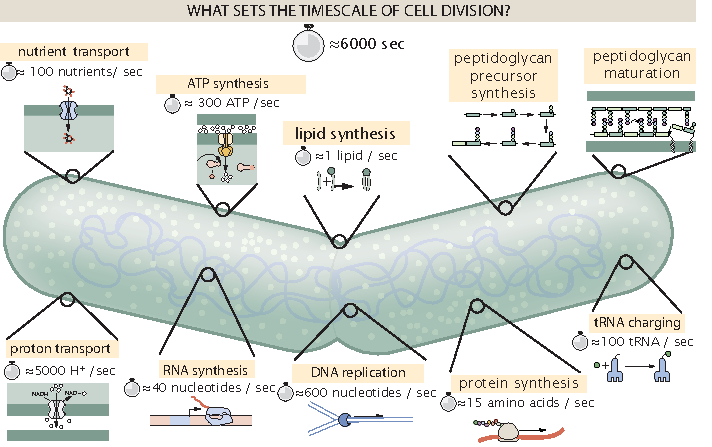
\includegraphics{main_figs/schematic_categories.pdf}
    \caption{\textbf{Transport and synthesis processes necessary for cell division.}
            We consider an array of processes necessary for a cell to double its
            molecular components. Such processes include the transport of carbon
            across the cell membrane, the production of ATP, and fundamental
            processes of the central dogma namely RNA, DNA, and protein
            synthesis. A schematic of each synthetic or transport category is
            shown with an estimate of the rate per macromolecular complex. In
            this work, we consider a standard bacterial division time of
            $\approx$ 6000 sec.}
    \label{fig:categories}
    }
\end{figure}
